% ============================================================
% Chapter 9 — The rotating ring
%
% Original work of this thesis. The material was developed for the
% first of the board models introduced in Section~\ref{sec:dev-board}
% and is reported here for the first time; there is no external source
% to cite for the derivations, the diagnostics, or the measurements.
% Numerical values are those of research/experiment1-rotating-ring/data.
% ============================================================

\chapter{The rotating ring: a two-dimensional dynamic object}
\label{ch:ring}

Chapters~\ref{ch:gaussian} and~\ref{ch:laplace} studied a chain of scalar
frames, where the joint score is either exactly Gaussian or a controlled
departure from it. Section~\ref{sec:dev-board} recorded a second family of
dynamic objects proposed in supervision, planar trajectories near a circle,
and set them aside because they are nonlinear in the coordinates in which the
diffusion acts. This chapter returns to the first of them. It shows that a
Cartesian surrogate of the model is exactly solvable, that the model as drawn
is solvable numerically to a measured accuracy, and that both admit the same
structural description of the joint score.

The question the chapter answers is narrower than the models it uses.

\begin{quote}
How can the Markov structure of the clean rotating trajectory be exploited to
compute and interpret the joint diffusion score?
\end{quote}

Four measurable subquestions make this operational: how far the joint score
differs from a collection of one-frame marginal scores; how strongly the
observation at frame $j$ influences the score block at frame $k$; how that
influence decays with the temporal lag $|j-k|$; and how many neighbouring
frames are needed to reproduce the score block to a stated accuracy. Every
answer below is a statement about one model at one parameter set, in the sense
fixed in Section~\ref{sec:rq}.

\section{Model and notation}\label{sec:ring-model}

\subsection{The clean process}

The clean state is a radius and a phase, evolving in the internal time $u$ as
two independent diffusions,
\begin{align}
  \dd R_u &= -\kappa (R_u - 1)\,\dd u + \sqrt{2 D_r}\, \dd B_u^{(r)} ,
  \label{eq:ring-radial-sde} \\
  \dd \Theta_u &= \omega\, \dd u + \sqrt{2 D_\theta}\, \dd B_u^{(\theta)} ,
  \label{eq:ring-angular-sde}
\end{align}
observed through the polar embedding
\begin{equation}
  a_u = R_u \big(\cos\Theta_u,\ \sin\Theta_u\big) \in \R^2 .
  \label{eq:ring-embedding}
\end{equation}
We use the simplest constant-angular-drift reading of the model;
Section~\ref{sec:ring-limits} records the alternatives.

A point of $\R^2$ is described by its distance from the origin and the angle it
makes with the first axis, and at each point the plane carries the orthonormal
moving frame
\begin{equation}
  e_r = (\cos\theta,\ \sin\theta), \qquad
  e_\theta = (-\sin\theta,\ \cos\theta) ,
  \label{eq:ring-moving-frame}
\end{equation}
in which $e_\theta$ is $e_r$ turned by a quarter revolution. Moving along $e_r$
changes the radius at fixed angle, moving along $e_\theta$ changes the angle at
fixed radius, and the area element is $\dd x\,\dd y = r\,\dd r\,\dd\theta$. The
decomposition matters because the two directions are treated very differently
by \eqref{eq:ring-radial-sde} and \eqref{eq:ring-angular-sde}: the radius is
pulled back towards one, the phase drifts and diffuses freely. Measuring the
consequence of that asymmetry for the score is one purpose of the chapter.

\subsection{The radial drift is a confining force}

Equation~\eqref{eq:ring-radial-sde} is the overdamped Langevin equation
\eqref{eq:langevin-sde} for the quadratic potential
\begin{equation}
  V(r) = \tfrac{\kappa}{2}\,(r-1)^2 .
  \label{eq:ring-potential}
\end{equation}
A potential stores energy, and the force it generates is minus its slope,
\begin{equation}
  F(r) = -V'(r) = -\kappa\,(r-1) .
  \label{eq:ring-force}
\end{equation}
The sign carries the content: a system driven by $-V'$ moves downhill in $V$,
since $\tfrac{\dd}{\dd u} V(r_u) = V'(r)\,\dot r = -V'(r)^2 \le 0$. Reading the
two cases of \eqref{eq:ring-force}, if $r > 1$ then $F < 0$ and the force points
inward, and if $r < 1$ then $F > 0$ and it points outward. The radius is driven
towards one from either side at a rate proportional to the displacement, with
$\kappa$ setting the stiffness. By \eqref{eq:langevin-boltzmann} the stationary
radial law is $\Nd(1, D_r/\kappa)$.

\subsection{One trajectory is one data point}

The trajectory is sampled at internal times $u_k = k h$ for
$k = 0, \dots, K-1$, and the complete datum is the stacked vector
\begin{equation}
  a = (a_0, a_1, \dots, a_{K-1}) \in \R^{2K} .
  \label{eq:ring-datum}
\end{equation}
The $K$ frames are correlated coordinates of one data point, not $K$ samples.
Relative to Chapter~\ref{ch:gaussian} the only change of setting is that each
frame is now two-dimensional, so the score has $K$ blocks of size two rather
than $K$ scalar components; the forward channel is unchanged,
\begin{equation}
  x = e^{-t} a + \sqrt{\Deltat}\, \xi , \qquad \xi \sim \Nd(0, I_{2K}) ,
  \label{eq:ring-channel}
\end{equation}
which is the channel of Section~\ref{sec:ou} acting on all $2K$ coordinates at
once. Figure~\ref{fig:ring-model} shows the model and the two clocks: internal
time orders the frames along the path, diffusion time corrupts them
simultaneously.

\begin{figure}[t]\centering
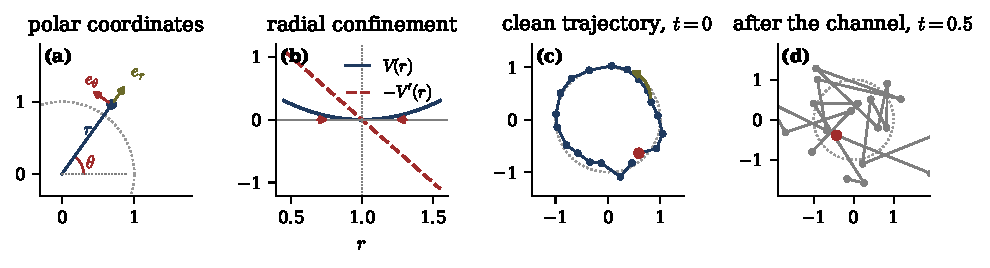
\includegraphics[width=\linewidth]{figures/fig_ring_model.pdf}
\caption{The rotating-ring model, at the parameters used throughout this
chapter ($K = 20$, $\kappa = 2$, $D_r = 0.015$, $D_\theta = 0.005$,
$\omega = 1$, $h = 2\pi/20$). (a) Polar coordinates and the moving frame
\eqref{eq:ring-moving-frame}. (b) The potential \eqref{eq:ring-potential} and
the force \eqref{eq:ring-force} it generates; the force changes sign at
$r = 1$, which is therefore the stable radius. (c) One clean trajectory, a
noisy coherently turning path near the unit circle; the arrow marks the sense
of rotation. (d) The same trajectory after the channel
\eqref{eq:ring-channel} at $t = 0.5$, from a single standardised noise
realisation.}
\label{fig:ring-model}
\end{figure}

\section{Two identities for the joint score}\label{sec:ring-identities}

The score--posterior identity of Section~\ref{sec:tweedie} applies unchanged.
Written per block, with the expectation taken under the posterior of the clean
trajectory given the whole noisy one,
\begin{equation}
  \score_k(x,t)
  = \frac{e^{-t}\,\E[a_k \,|\, x_0, \dots, x_{K-1}] - x_k}{\Deltat}
  \ \in \R^2 .
  \label{eq:ring-block-score}
\end{equation}
The score block at frame $k$ is a \emph{smoothing} estimate: it uses every
observation, before and after $k$, to estimate one clean frame. Two
consequences of \eqref{eq:ring-block-score} are used repeatedly and are derived
here.

\subsection{The joint and marginal objects differ by a conditioning set}

The one-frame marginal score denoises frame $k$ from frame $k$ alone,
\begin{equation}
  s^{\mathrm{marg}}_k(x_k, t)
  = \frac{e^{-t}\,\E[a_k \,|\, x_k] - x_k}{\Deltat} ,
  \label{eq:ring-marg-score}
\end{equation}
and subtracting it from \eqref{eq:ring-block-score} isolates the difference
exactly:
\begin{equation}
  \boxed{\;
  \score_k(x,t) - s^{\mathrm{marg}}_k(x_k,t)
  = \frac{e^{-t}}{\Deltat}
    \Big( \E[a_k \,|\, x_{0:K-1}] - \E[a_k \,|\, x_k] \Big) \; }
  \label{eq:ring-gap}
\end{equation}
The gap is the extra denoising information supplied by the rest of the
trajectory, and nothing else. Figure~\ref{fig:ring-joint-marg} states the same
thing as a graphical model, in the form used in Chapter~\ref{ch:graphs}: the
joint score is a smoother, in which every observation has a path to every clean
frame, whereas the product-of-marginals score severs all cross-frame paths
before denoising begins.

\begin{figure}[t]\centering
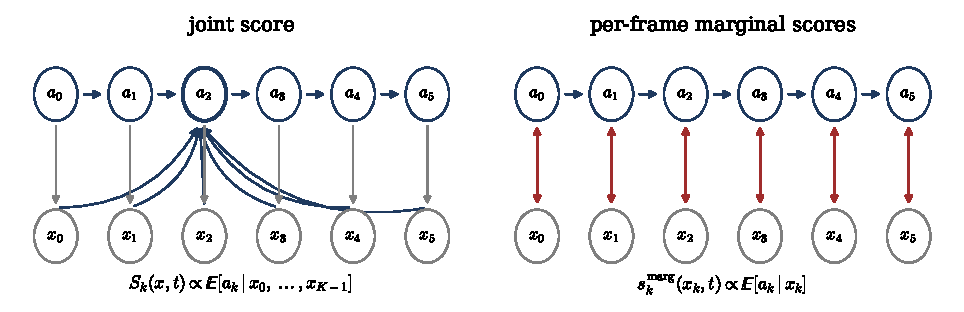
\includegraphics[width=\linewidth]{figures/fig_ring_joint_vs_marginal.pdf}
\caption{The two objects compared in \eqref{eq:ring-gap}. Clean frames $a_k$
form a Markov chain in internal time and each emits one noisy observation
$x_k$ through the channel \eqref{eq:ring-channel}. Left: computing
$\score_2$ requires the posterior of $a_2$ given all observations, so every
$x_j$ has a path to $a_2$. Right: the per-frame marginal score conditions on
$x_k$ alone. The magnitude of the difference is measured in
Sections~\ref{sec:ring-surrogate-measurements} and~\ref{sec:ring-measurements}.}
\label{fig:ring-joint-marg}
\end{figure}

\subsection{The response of the score is a posterior covariance}
\label{sec:ring-response}

The second subquestion asks how strongly the observation at frame $j$
influences the score block at frame $k$. The answer is an exact identity, and
every quantity measured later in the chapter is an instance of it.

\begin{toolbox}[tb:ring-response]{The observation as an external field}
\textbf{Step 1: write the posterior as a Gibbs measure with a linear field.}
By Bayes and \eqref{eq:ring-channel},
\begin{align*}
  p(a \,|\, x)
  &\propto P_0(a)\, \exp\!\Big[ -\frac{\norm{x - e^{-t} a}^2}{2\Deltat} \Big] \\
  &= P_0(a)\,
     \underbrace{\exp\!\Big[-\frac{\norm{x}^2}{2\Deltat}\Big]}_{\text{no } a}
     \exp\!\Big[ -\frac{e^{-2t}}{2\Deltat}\norm{a}^2
                 + \frac{e^{-t}}{\Deltat}\, x^{\T} a \Big] \\
  &\propto
     \underbrace{P_0(a)\,
       \exp\!\Big[-\frac{e^{-2t}}{2\Deltat}\norm{a}^2\Big]}_{
       \textstyle \nu(a),\ \text{independent of } x}
     \; e^{\, h^{\T} a} ,
  \qquad
  h = \frac{e^{-t}}{\Deltat}\, x .
\end{align*}
Expanding $\norm{x - e^{-t}a}^2$ produces exactly three kinds of term: one free
of $a$, absorbed by the normalisation; one quadratic in $a$ and free of $x$;
and one bilinear term. The whole dependence on the data therefore enters
through a single vector $h$ coupled \emph{linearly} to $a$. In the language of
Section~\ref{sec:free-energy}, the observation at frame $j$ acts as an external
field $h_j = (e^{-t}/\Deltat)\,x_j$ conjugate to the clean state $a_j$.

\textbf{Step 2: differentiate the log-normalisation once.} With
$Z(h) = \int \nu(a)\, e^{h^{\T} a}\,\dd a$, so that
$p(a\,|\,x) = \nu(a) e^{h^{\T}a}/Z(h)$,
\begin{equation}
  \frac{\partial \log Z}{\partial h_j}
  = \frac{1}{Z}\int a_j\, \nu(a)\, e^{h^{\T}a}\, \dd a
  = \E[a_j \,|\, x] .
  \label{eq:ring-cumulant-1}
\end{equation}
$\log Z$ is the cumulant generating function of the posterior.

\textbf{Step 3: differentiate twice.} Differentiating
\eqref{eq:ring-cumulant-1} again, using
$\partial_{h_k} e^{h^{\T}a} = a_k e^{h^{\T}a}$ and
$\partial_{h_k} Z^{-1} = -Z^{-2}\partial_{h_k} Z$,
\begin{equation}
  \frac{\partial^2 \log Z}{\partial h_k \partial h_j}
  = \E[a_k a_j \,|\, x] - \E[a_k\,|\,x]\,\E[a_j\,|\,x]
  = \mathrm{Cov}(a_k, a_j \,|\, x) ,
  \label{eq:ring-cumulant-2}
\end{equation}
so that the derivative of a posterior mean with respect to the field is a
posterior covariance,
$\partial_{h_j} \E[a_k\,|\,x] = \mathrm{Cov}(a_k, a_j\,|\,x)$.

\textbf{Step 4: change variables back to the data.} Since
$h = (e^{-t}/\Deltat)\, x$, the chain rule gives
$\partial/\partial x_j = (e^{-t}/\Deltat)\,\partial/\partial h_j$ and
\begin{equation}
  \frac{\partial}{\partial x_j}\E[a_k \,|\, x]
  = \frac{e^{-t}}{\Deltat}\, \mathrm{Cov}(a_k, a_j \,|\, x) .
  \label{eq:ring-mean-response}
\end{equation}

\textbf{Step 5: differentiate the score.} Apply $\partial/\partial x_j$ to
\eqref{eq:ring-block-score}. The posterior mean contributes
$(e^{-t}/\Deltat)$ times \eqref{eq:ring-mean-response}, the subtracted $x_k$
contributes $-\delta_{kj} I_2 / \Deltat$, which gives
\eqref{eq:ring-fdt}. \hfill$\square$
\end{toolbox}

\begin{proposition}[Posterior response identity]\label{prop:ring-fdt}
For every pair of frames $k, j$ and every $t > 0$,
\begin{equation}
  \boxed{\;
  J_{kj}(x,t) := \frac{\partial \score_k}{\partial x_j}
  = -\frac{\delta_{kj}}{\Deltat}\, I_2
    + \frac{e^{-2t}}{\Deltat^2}\,
      \mathrm{Cov}\big(a_k, a_j \,\big|\, x\big) \; }
  \label{eq:ring-fdt}
\end{equation}
where $\mathrm{Cov}(a_k, a_j \,|\, x) \in \R^{2\times2}$ is the
cross-covariance block of the two clean frames under the posterior given the
whole noisy trajectory.
\end{proposition}

Two remarks fix the status of \eqref{eq:ring-fdt}. First, it is a consistency
check on itself: $J$ is the Hessian $\nabla^2 \log P_t$, so it must be
symmetric under exchanging the pairs $(k,\alpha)$ and $(j,\beta)$, and it is,
because transposing the block of \eqref{eq:ring-fdt} exchanges $a_k$ and $a_j$.
Second, it is the static linear-response relation of
Section~\ref{sec:free-energy}: a derivative with respect to a field equals a
covariance in one fixed measure. It is not a two-time dynamical
fluctuation--dissipation theorem, and none is claimed.

For $j \ne k$ the response is proportional to a posterior cross-covariance.
Perturbing a distant observed frame changes $\score_k$ if and only if the two
clean states remain statistically coupled \emph{after} conditioning on the
whole noisy trajectory. The pattern of the score Jacobian is therefore a map of
posterior information flow, and the prefactor $e^{-2t}/\Deltat^2$, which tends
to zero as $t$ grows, is separate from that pattern. Keeping the two apart is
the purpose of the next section.

\section{Diagnostics}\label{sec:ring-diagnostics}

Subquestions two to four concern strength, reach, and sufficiency. These are
three properties of one profile, and in the measurements below they move in
different directions with diffusion time. Fix a central frame $k$ and let
\begin{equation}
  C_t(\ell) = \E_x\big[ \norm{J_{k,k+\ell}(x,t)}_F \big] ,
  \qquad \ell = 0, 1, \dots, L_{\max} ,
  \label{eq:ring-profile}
\end{equation}
be the \emph{response profile}: the mean Frobenius norm of the response block
at lag $\ell$, averaged over noisy trajectories and over the two sides
$k \pm \ell$. By \eqref{eq:ring-fdt} the self-response $C_t(0)$ is dominated by
$1/\Deltat$.

\paragraph{Strength.} The total cross-frame response is
\begin{equation}
  I_{\mathrm{off}}(t) = \sum_{\ell \ge 1} C_t(\ell) .
  \label{eq:ring-intensity}
\end{equation}
It answers how much the other frames matter in total, and says nothing about
where they sit.

\paragraph{Reach.} The natural first choice is an e-folding length obtained by
fitting $C_t(\ell) \approx C_t(1)\exp[-(\ell-1)/\xi^{\mathrm{exp}}]$. It is the
finite-chain estimate of a correlation length, and in the low-noise regime it
is informative. It is also unbounded: once the measured profile is nearly flat
the fit is ill-conditioned, and in our measurements the fitted
$\xi^{\mathrm{exp}}_\theta$ exceeds $290$ frames in a chain of $20$ at the
largest diffusion times. We therefore report it only where it is meaningful,
and use as the working measure of reach the first moment of the response mass,
\begin{equation}
  \bar\ell(t)
  = \frac{\sum_{\ell \ge 1} \ell\, C_t(\ell)}{\sum_{\ell \ge 1} C_t(\ell)} ,
  \label{eq:ring-mean-lag}
\end{equation}
the centre of mass of the cross-frame response. It is measured in frames, is
bounded by $L_{\max}$, and assumes no particular shape of profile. It has a
known \emph{structureless ceiling}: a flat profile gives
$\bar\ell = (1 + L_{\max})/2$, which is $5.5$ for the $L_{\max} = 10$ of this
chapter. A measured $\bar\ell$ near $5.5$ therefore indicates that the temporal
structure has been erased, not that the correlation is long. The same caveat
applies to the shape-only normalised range
$\xi^{\mathrm{norm}}(t) = \sum_{\ell\ge1} C_t(\ell)/C_t(1)$, whose ceiling is
$L_{\max}$, and which by construction cannot distinguish a strong short-range
coupling from a negligible long-range one.

\paragraph{Strength and reach together.} Intensity and mean lag answer
complementary questions, and their product is a single number that responds to
either:
\begin{equation}
  \Xi(t) = I_{\mathrm{off}}(t)\, \bar\ell(t)
         = \sum_{\ell\ge1} \ell\, C_t(\ell) ,
  \qquad
  \boxed{\ \widetilde\Xi(t) = \frac{\Xi(t)}{C_t(0)}\ }
  \label{eq:ring-weighted-reach}
\end{equation}
$\Xi$ is the unnormalised first moment of the profile: it increases if the
coupling becomes stronger or if it arrives from farther away, and it factorises
exactly into how much times how far, so the two ingredients can always be read
off separately. Dividing by the self-response makes it comparable across
diffusion times, since $C_t(0) \simeq 1/\Deltat$ removes the overall scale of
the Jacobian, and leaves a quantity measured in frames that expresses the reach
of the context relative to the local term competing with it. Like $\bar\ell$ it
inherits a ceiling and must be read against it.

\paragraph{Sufficiency.} Every diagnostic so far is infinitesimal. A direct
test of the fourth subquestion is to recompute the score block from a truncated
window $x_{k-L:k+L}$, ignoring the rest of the trajectory. Writing
$\score^{(L)}_k$ for that windowed score,
\begin{equation}
  \varepsilon_L(t)
  = \left[
      \frac{\E \norm{\score^{(L)}_k - \score^{\mathrm{full}}_k}^2}
           {\E \norm{\score^{\mathrm{full}}_k}^2}
    \right]^{1/2} ,
  \qquad
  L_\epsilon(t) = \min\{ L : \varepsilon_L(t) \le \epsilon \} .
  \label{eq:ring-window}
\end{equation}
$L_\epsilon$ carries the most direct modelling reading of the four, in the sense
of Section~\ref{sec:cnn-locality}: it is the temporal window a denoiser would
need in order to reproduce the score to accuracy $\epsilon$ at that noise
level. It is also the most expensive to compute, which is why the
infinitesimal diagnostics are worth having.

\begin{remark}[What a large reach does not imply]\label{rem:ring-ceiling}
If every off-diagonal response is small but nearly equal, then
$\xi^{\mathrm{norm}}$ and $\bar\ell$ both saturate at their structureless
ceilings while the total correction to the score is negligible. That is what
occurs at large diffusion time, where the score approaches the field $-x$.
Conversely $I_{\mathrm{off}}$ alone cannot separate a tightly local coupling
from a diffuse one. Only the pair, or the weighted reach that combines them, is
safe to quote, and no diagnostic here should be read as an infinite-volume
correlation length: $K = 20$ is finite and no thermodynamic limit is taken.
\end{remark}

\section{An exactly solvable surrogate}\label{sec:ring-surrogate}

\subsection{The surrogate, and what it keeps}

The surrogate retains a ring, a coherent rotation, and dependence along the
trajectory, and drops the rest:
\begin{align}
  z_0 &\sim p_\lambda(z) \propto
        \exp\!\Big[-\frac{(\norm{z}-1)^2}{2\lambda}\Big] ,
  \label{eq:ring-sur-prior} \\
  z_{k+1} &= R_\psi z_k + \sigma \eta_{k+1} ,
        \qquad \eta_{k+1} \stackrel{\text{iid}}{\sim} \Nd(0, I_2) ,
  \label{eq:ring-sur-dynamics}
\end{align}
with $R_\psi$ the planar rotation through the one-frame angle
$\psi = \omega h$.

\begin{remark}[The surrogate is not a discretisation of the polar model]
\label{rem:ring-surrogate-scope}
In \eqref{eq:ring-sur-dynamics} the ring acts only on $z_0$. Later frames form
a rotating Cartesian random walk and their radial variance grows without bound,
whereas in \eqref{eq:ring-radial-sde} a confining force acts at every internal
time. The surrogate is a solvable companion whose role is to exhibit the
mechanism in closed form, not to approximate the model of
Section~\ref{sec:ring-model}.
\end{remark}

\subsection{The known rotation is an orthogonal change of frame}

The rotation is the object to be removed, so we write it out:
\begin{equation}
  R_\psi =
  \begin{pmatrix} \cos\psi & -\sin\psi \\ \sin\psi & \cos\psi \end{pmatrix} .
  \label{eq:ring-rotation}
\end{equation}
Its columns are the standard basis vectors, each turned through $\psi$. They
are unit vectors, since $\cos^2\psi + \sin^2\psi = 1$, and orthogonal, since
$\cos\psi(-\sin\psi) + \sin\psi\cos\psi = 0$. In matrix form,
\begin{equation}
  R_\psi^{\T} R_\psi = I_2, \qquad \det R_\psi = 1, \qquad
  R_\psi^{\T} = R_{-\psi}, \qquad R_\psi R_\varphi = R_{\psi+\varphi} ,
  \label{eq:ring-rot-props}
\end{equation}
and orthogonality gives
$\norm{R_\psi z}^2 = z^{\T} R_\psi^{\T} R_\psi z = \norm{z}^2$: lengths and
inner products are preserved.

\begin{lemma}[Rotations preserve the standard isotropic Gaussian]
\label{lem:ring-isotropy}
If $\eta \sim \Nd(0, I_2)$ and $R$ is orthogonal, then $R\eta \sim \Nd(0,I_2)$.
\end{lemma}

\begin{proof}
A linear map of a Gaussian is Gaussian, so $R\eta$ is fixed by its first two
moments: $\E[R\eta] = R\,\E[\eta] = 0$ and
$\mathrm{Cov}(R\eta) = R\, I_2\, R^{\T} = R R^{\T} = I_2$. Equivalently, in
terms of densities, $(2\pi)^{-1}e^{-\norm{z}^2/2}$ depends on $z$ only through
$\norm{z}$, and the change of variables $z \mapsto Rz$ changes neither
$\norm{R^{-1}z} = \norm{z}$ nor $|\det R^{-1}| = 1$: the level sets are circles
centred at the origin and a rotation maps each circle to itself.
\end{proof}

The isotropy is essential. A rotation would not preserve $\Nd(0,\Sigma)$ for
general $\Sigma$, and the reduction below is exact only because both the
innovation in \eqref{eq:ring-sur-dynamics} and the channel
\eqref{eq:ring-channel} are isotropic.

\begin{lemma}[Gauge reduction]\label{lem:ring-gauge}
Define the de-rotated frame $y_k = R_{-k\psi} z_k$ and stack the per-frame
rotations into
$U_\psi = \mathrm{diag}(I_2, R_{-\psi}, \dots, R_{-(K-1)\psi})$. Then
\begin{equation}
  y_{k+1} = y_k + \sigma \widetilde\eta_{k+1} ,
  \qquad \widetilde\eta_{k+1} \stackrel{\text{iid}}{\sim} \Nd(0, I_2) ,
  \label{eq:ring-gauged-rw}
\end{equation}
$U_\psi$ is orthogonal, and the noised density and score satisfy
\begin{equation}
  P_t(z \,|\, \psi) = P^{(0)}_t(U_\psi z) ,
  \qquad
  \score_\psi(z,t) = U_\psi^{\T}\, \score^{(0)}(U_\psi z, t) ,
  \label{eq:ring-gauge-score}
\end{equation}
where the superscript zero denotes the quantities of the non-rotating model.
\end{lemma}

\begin{proof}
Substituting \eqref{eq:ring-sur-dynamics} and using the composition rule of
\eqref{eq:ring-rot-props},
\begin{equation*}
  y_{k+1}
  = R_{-(k+1)\psi}\big(R_\psi z_k + \sigma\eta_{k+1}\big)
  = \underbrace{R_{-(k+1)\psi}R_\psi}_{= R_{-k\psi}} z_k
    + \sigma R_{-(k+1)\psi}\eta_{k+1}
  = y_k + \sigma\widetilde\eta_{k+1} ,
\end{equation*}
and by Lemma~\ref{lem:ring-isotropy} each
$\widetilde\eta_{k+1} \sim \Nd(0,I_2)$; they stay independent because each is a
fixed linear map of a different independent $\eta$. Next, $U_\psi$ is block
diagonal with orthogonal blocks, so
$U_\psi^{\T} U_\psi = \mathrm{diag}(I_2, \dots, I_2) = I_{2K}$ and
$\det U_\psi = \prod_k \det R_{-k\psi} = 1$. Applying $U_\psi$ to
\eqref{eq:ring-channel} gives
$U_\psi x = e^{-t} U_\psi a + \sqrt{\Deltat}\, U_\psi \xi$ with
$U_\psi \xi \sim \Nd(0, I_{2K})$, so $U_\psi x$ has exactly the law of the
noised non-rotating trajectory: the de-rotation commutes with the channel. For
the densities, $z = U_\psi^{\T} y$ and
$P_t(z\,|\,\psi) = P^{(0)}_t(U_\psi z)\,|\det U_\psi|$, the Jacobian factor
being one. Differentiating that identity componentwise, with
$\partial y_b/\partial z_c = (U_\psi)_{bc}$,
\begin{equation*}
  \frac{\partial}{\partial z_c} \log P^{(0)}_t(U_\psi z)
  = \sum_b (U_\psi)_{bc}\,
    \big(\nabla \log P^{(0)}_t\big)_b (U_\psi z)
  = \big[ U_\psi^{\T} \score^{(0)}(U_\psi z, t) \big]_c .
\end{equation*}
The transpose is not cosmetic: a score is a gradient, so it transforms with
$U_\psi^{\T}$ while a point transforms with $U_\psi$.
\end{proof}

The term \emph{gauge} is used in the sense standard in physics, of a change of
description that leaves the content untouched and may be chosen to simplify the
equations. Equation~\eqref{eq:ring-gauge-score} says that a known rotation adds
no statistical difficulty: de-rotate the data, solve the non-rotating problem,
rotate the score back. Since $U_\psi^{\T} = U_\psi^{-1}$, the operation is
exactly invertible and destroys no information. It would not hold for an
\emph{unknown} $\psi$, which is a genuine latent variable
(Section~\ref{sec:ring-limits}). Figure~\ref{fig:ring-gauge} shows the two
frames.

\begin{figure}[t]\centering
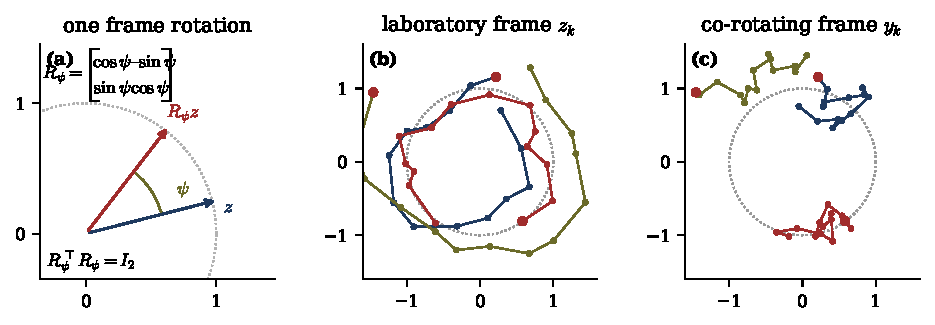
\includegraphics[width=\linewidth]{figures/fig_ring_gauge.pdf}
\caption{The rotation and the gauge. (a) $R_\psi$ turns every vector through
the same angle without changing its length, which is the statement
$R_\psi^{\T}R_\psi = I_2$. (b) Three surrogate trajectories in the laboratory
frame ($K = 14$, $\sigma = 0.16$, $\psi = 2\pi/14$; the marked point is
$k = 0$), coherently circulating. (c) The same trajectories after $U_\psi$: a
random walk anchored on the ring. Because $U_\psi$ is orthogonal the reduction
is exact at every diffusion time; the numerical round trip agrees to machine
precision (Table~\ref{tab:ring-validation}).}
\label{fig:ring-gauge}
\end{figure}

\subsection{The clean law after the gauge}

Iterating \eqref{eq:ring-gauged-rw} and letting the intermediate terms cancel,
\begin{equation}
  y_k - y_0 = \sum_{r=1}^{k} (y_r - y_{r-1})
            = \sigma \sum_{r=1}^{k} \widetilde\eta_r ,
  \qquad\text{so}\qquad
  y_k = A + \sigma \sum_{r=1}^{k} \widetilde\eta_r ,
  \label{eq:ring-unrolled}
\end{equation}
with $A := y_0 \sim p_\lambda$ and the empty sum equal to zero. Every frame
contains the \emph{same} random anchor, drawn once on the ring, plus a partial
sum of independent innovations; the anchor is the only non-Gaussian ingredient
of the model.

The clean law factorises over the ring prior and the one-step transitions, so
$\log P_0(y) = -(\norm{y_0}-1)^2/2\lambda
- (2\sigma^2)^{-1}\sum_{k=0}^{K-2}\norm{y_{k+1}-y_k}^2 + \text{const}$.
Differentiating is a counting exercise: an interior $y_k$ appears in exactly two
summands, the edge arriving at it and the edge leaving it, whose derivatives are
$-(y_k - y_{k-1})/\sigma^2$ and $+(y_{k+1} - y_k)/\sigma^2$. Adding them, and
using $\nabla_y \norm{y} = y/\norm{y}$ for the ring term,
\begin{align}
  \score_0(y,0)
    &= \frac{1-\norm{y_0}}{\lambda}\,\frac{y_0}{\norm{y_0}}
       + \frac{y_1 - y_0}{\sigma^2},
  \notag \\
  \score_k(y,0)
    &= \frac{y_{k-1} - 2y_k + y_{k+1}}{\sigma^2},
       \qquad 1 \le k \le K-2,
  \label{eq:ring-clean-score} \\
  \score_{K-1}(y,0)
    &= \frac{y_{K-2}-y_{K-1}}{\sigma^2} .
  \notag
\end{align} The interior clean score is a
discrete second derivative along internal time, that is a discrete Laplacian:
each block measures how far frame $k$ departs from the average of its
neighbours. It is strictly local, and it vanishes identically on the model's
own noiseless solution, because a trajectory rotating at radius exactly one
maps under the gauge to a constant $y_k$, for which every second difference
vanishes and, with $\norm{y_0} = 1$, so does the ring term. That vanishing is
verified to machine zero (Table~\ref{tab:ring-validation}).

\subsection{The noised law and the exact score}

Conditioning on the anchor, \eqref{eq:ring-unrolled} gives
$\E[y_i \,|\, A = \alpha] = \alpha$ and
\begin{equation}
  \mathrm{Cov}(y_i, y_j \,|\, A)
  = \sigma^2\, \E\Big[\Big(\textstyle\sum_{r \le i}\widetilde\eta_r\Big)
      \Big(\textstyle\sum_{s \le j}\widetilde\eta_s\Big)^{\!\T}\Big]
  = \sigma^2 \min(i,j)\, I_2 ,
  \label{eq:ring-K}
\end{equation}
since $\E[\widetilde\eta_r \widetilde\eta_s^{\T}] = \delta_{rs} I_2$ leaves only
the $\min(i,j)$ indices common to both sums. Compactly,
$y \,|\, A = \alpha \sim \Nd(\mathbf{1} \otimes \alpha,\ G \otimes I_2)$
with $G_{ij} = \sigma^2\min(i,j)$, where $\mathbf 1 \in \R^K$ is the
all-ones vector. The two Kronecker products separate the temporal index from
the spatial one: $\mathbf 1 \otimes \alpha$ repeats the same two-dimensional
anchor in every frame, and
$(G \otimes I_2)_{(i,\alpha'),(j,\beta')}
= G_{ij}\,\delta_{\alpha'\beta'}$, so $G$ carries all the temporal
correlation while $I_2$ states that the two spatial coordinates are
uncorrelated and share the same temporal covariance. Applying the channel and
using $I_{2K} = I_K \otimes I_2$ to combine the covariances,
\begin{equation}
  x \,|\, A = \alpha
  \ \sim\ \Nd\big(e^{-t}\,\mathbf 1 \otimes \alpha,\ C_t \otimes I_2\big),
  \qquad
  C_t = e^{-2t}G + \Deltat\, I_K ,
  \label{eq:ring-Ct}
\end{equation}
in which $C_t$ does not depend on $\alpha$: the noised law is a two-parameter
location mixture of one fixed Gaussian.

\begin{proposition}[Exact surrogate score and response]\label{prop:ring-exact}
Let $q = C_t^{-1}\mathbf 1$, $\beta = e^{-2t}\mathbf 1^{\T} C_t^{-1}\mathbf 1$
and $h = e^{-t}\sum_j q_j x_j \in \R^2$. Then the anchor posterior is
\begin{equation}
  p(\alpha \,|\, x) \propto
  \exp\!\Big[ -\frac{(\norm{\alpha}-1)^2}{2\lambda}
              - \frac{\beta}{2}\norm{\alpha}^2 + h^{\T}\alpha \Big] ,
  \label{eq:ring-anchor-posterior}
\end{equation}
and the score and response blocks are
\begin{equation}
  \score_k(x,t) = -\big(C_t^{-1}x\big)_k + e^{-t} q_k\, \E[A \,|\, x] ,
  \qquad
  J_{kj}(x,t) = -\big(C_t^{-1}\big)_{kj} I_2
                + e^{-2t}\, q_k q_j\, \mathrm{Cov}(A \,|\, x) .
  \label{eq:ring-surrogate-score}
\end{equation}
\end{proposition}

\begin{proof}
Expanding the exponent of \eqref{eq:ring-Ct} in powers of $\alpha$, as in Step~1
of Toolbox~\ref{tb:ring-response} but with the correlated covariance
$C_t \otimes I_2$, gives \eqref{eq:ring-anchor-posterior}. Writing
$\log P_t(x) = \text{const} - \tfrac12 x^{\T}(C_t^{-1}\otimes I_2)x
+ \log Z(h(x))$, the gradient of the first term is $-(C_t^{-1}x)_k$ in block
$k$, while $\partial h/\partial x_k = e^{-t}q_k I_2$ and
$\nabla_h \log Z = \E[A\,|\,x]$ by \eqref{eq:ring-cumulant-1}. Differentiating
once more and using \eqref{eq:ring-cumulant-2} gives the response.
\end{proof}

The $2K$-dimensional integral over clean trajectories has collapsed to a
two-dimensional posterior over the shared anchor, which is the whole
simplification and a direct consequence of \eqref{eq:ring-unrolled}. Its two
moments are cheap: the prior and the $\norm{\alpha}^2$ term are rotationally
symmetric, so the posterior depends on the direction of $\alpha$ only through
$h^{\T}\alpha$, and
$\E[A\,|\,x] = \mu(\norm{h})\,\widehat h$ with
$\mathrm{Cov}(A\,|\,x) = v_\perp I_2 + (v_\parallel - v_\perp)
\widehat h \widehat h^{\T}$, three scalar functions of one scalar argument,
tabulated once per diffusion time by one-dimensional quadrature.

The structural content of \eqref{eq:ring-surrogate-score} is that the temporal
coefficient of the second term is the outer product $q q^{\T}$, which is of
rank one. The nonlocal part of the response is therefore not a chain of local
couplings but a single shared latent variable seen by every frame.
Figure~\ref{fig:ring-surrogate-response} separates the two terms.

\begin{figure}[t]\centering
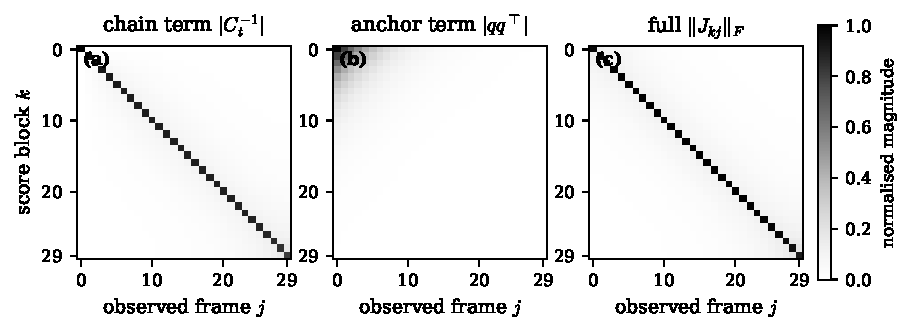
\includegraphics[width=\linewidth]{figures/fig_ring_surrogate_response.pdf}
\caption{Exact decomposition of the surrogate response
\eqref{eq:ring-surrogate-score} at $t = 0.20$, $K = 30$, $\lambda = 0.05$,
$\sigma = 0.15$, averaged over $250$ noisy trajectories, each panel normalised
by its own maximum. (a) The chain term $|C_t^{-1}|$ is concentrated near the
diagonal. (b) The anchor coefficient $|qq^{\T}|$ is rank one and spread over
all lags. (c) The mean norm of the complete $2\times2$ blocks. The analytic
Jacobian agrees with central finite differences to $9.2\times10^{-6}$
(Table~\ref{tab:ring-validation}).}
\label{fig:ring-surrogate-response}
\end{figure}

\begin{proposition}[What the surrogate establishes]
\label{prop:ring-surrogate-conclusion}
Clean Markov locality does not survive marginalisation through the OU channel
as locality of the noised score: by \eqref{eq:ring-surrogate-score} the
response has nonzero blocks at every lag for every $t > 0$. The nonlocal part
is nonetheless structured, decomposing exactly into a near-diagonal chain term
and a rank-one correction generated by the shared ring anchor.
\end{proposition}

\subsection{What the surrogate measures}\label{sec:ring-surrogate-measurements}

At $K = 30$, $\lambda = 0.05$, $\sigma = 0.15$, $\psi = 2\pi/30$, with $350$
clean trajectories corrupted independently at each diffusion time, the profile
\eqref{eq:ring-profile} is averaged over all frame pairs at equal lag, so
$L_{\max} = 29$ and the structureless ceilings are $\bar\ell = 15$ and
$\xi^{\mathrm{norm}} = 29$; the window error is measured at the central frame.
Table~\ref{tab:ring-surrogate} reports the result.

\begin{table}[t]\centering
\caption{Surrogate diagnostics. ``Marginal'' is the relative RMS error of
replacing the joint score by per-frame marginal scores, $I_{\mathrm{off}}$ the
intensity \eqref{eq:ring-intensity}, $\bar\ell$ the weighted mean lag
\eqref{eq:ring-mean-lag}, $\widetilde\Xi$ the relative weighted reach
\eqref{eq:ring-weighted-reach} and $L_{5\%}$ the receptive radius
\eqref{eq:ring-window}. The last row is the value a flat profile would give.}
\label{tab:ring-surrogate}
\begin{tabular}{@{}rrrrrr@{}}
\toprule
$t$ & marginal & $I_{\mathrm{off}}$ & $\bar\ell$ & $\widetilde\Xi$ & $L_{5\%}$ \\
\midrule
0.05 & 0.959 & 6.093 & 2.73 & 1.467 & 6 \\
0.20 & 0.779 & 2.177 & 5.34 & 3.067 & 10 \\
0.70 & 0.462 & 1.171 & 10.61 & 6.994 & 13 \\
1.50 & 0.154 & 0.703 & 13.30 & 6.430 & 11 \\
\midrule
\emph{flat} & --- & --- & 15.00 & --- & --- \\
\bottomrule
\end{tabular}
\end{table}

Three readings. First, the cost of dropping temporal context is largest at low
noise: at $t = 0.02$ the per-frame marginal score has a relative RMS error of
$0.977$, falling to $0.154$ at $t = 1.5$ and $0.011$ at $t = 3$. The decline
does not mean that the joint structure was unimportant at small $t$; it means
that at large $t$ the score itself approaches the field $-x$, which the
marginal object also reproduces. Second, reach and intensity move in opposite
directions: the intensity falls by a factor of $173$ between $t = 0.02$ and
$t = 3$, while $\bar\ell$ rises from $1.94$ to $13.9$ frames, that is from a
genuinely local profile to one close to flat. The composite $\widetilde\Xi$
resolves the two, rising to $7.7$ at $t = 1$ and falling afterwards. Third, the
receptive field is non-monotone in $t$: the radius required for $5\%$ accuracy
is $6, 10, 13, 11$ at $t = 0.05, 0.20, 0.70, 1.50$.

\section{The model as drawn}\label{sec:ring-polar}

The polar process of Section~\ref{sec:ring-model} has no gauge to remove, and
its one-step transitions must be computed. Both are exactly available because
each of \eqref{eq:ring-radial-sde} and \eqref{eq:ring-angular-sde} is linear.

\begin{toolbox}[tb:ring-radial]{The exact one-step radial law}
\textbf{Step 1: shift to the equilibrium radius.} Put $Y_u = R_u - 1$. Since
$1$ is constant, $\dd Y_u = \dd R_u$ and \eqref{eq:ring-radial-sde} becomes an
Ornstein--Uhlenbeck equation with no offset,
$\dd Y_u = -\kappa Y_u\,\dd u + \sqrt{2D_r}\,\dd B_u$.

\textbf{Step 2: multiply by the integrating factor $e^{\kappa u}$.} Take
$\phi(y,u) = e^{\kappa u}y$. It is linear in $y$, so
$\partial^2_y \phi = 0$ and It\^o's lemma (Toolbox~\ref{tb:ito-lemma}) reduces to the
ordinary product rule, with no correction term:
\begin{align*}
  \dd\big(e^{\kappa u} Y_u\big)
  &= \kappa e^{\kappa u} Y_u\,\dd u + e^{\kappa u}\,\dd Y_u \\
  &= \kappa e^{\kappa u} Y_u\,\dd u
     + e^{\kappa u}\big(-\kappa Y_u\,\dd u + \sqrt{2D_r}\,\dd B_u\big)
   = \sqrt{2D_r}\, e^{\kappa u}\, \dd B_u .
\end{align*}
The two drift terms cancel by construction, which is what the factor is chosen
for, and what remains is an exact differential free of $Y$.

\textbf{Step 3: integrate over one step.} Integrating from $u_k$ to
$u_{k+1} = u_k + h$, the left side telescopes to
$e^{\kappa u_{k+1}}Y_{k+1} - e^{\kappa u_k}Y_k$. Multiplying throughout by
$e^{-\kappa u_{k+1}}$, so that
$e^{-\kappa u_{k+1}}e^{\kappa u_k} = e^{-\kappa h}$ on the left, and carrying
the constant $e^{-\kappa u_{k+1}}$ inside the integral on the right,
\begin{equation}
  Y_{k+1} = e^{-\kappa h}\, Y_k
    + \sqrt{2D_r} \int_{u_k}^{u_{k+1}}
      e^{-\kappa(u_{k+1}-s)}\, \dd B_s .
  \label{eq:ring-radial-solution}
\end{equation}
The kernel is deterministic and weights the noise injected at time $s$ by how
much of it survives to $u_{k+1}$.

\textbf{Step 4: the stochastic integral has mean zero.} In the defining sum of
Section~\ref{sec:ode-to-sde} each term is
$f(s_i)\,(B_{s_{i+1}} - B_{s_i})$ with $f(s) = e^{-\kappa(u_{k+1}-s)}$ a fixed
number and the increment independent of the past with mean zero, so every term
has mean zero and so does the limit. Hence
$\E[Y_{k+1}\,|\,Y_k] = e^{-\kappa h}Y_k$: the conditional mean relaxes
geometrically towards zero, that is $R$ relaxes towards one.

\textbf{Step 5: its variance, by the It\^o isometry.} With the same
deterministic $f$, and substituting $v = u_{k+1}-s$ so that the limits
$s = u_k, u_{k+1}$ become $v = h, 0$,
\begin{equation}
  2D_r \int_{u_k}^{u_{k+1}} e^{-2\kappa(u_{k+1}-s)}\,\dd s
  = 2D_r \int_0^h e^{-2\kappa v}\,\dd v
  = \frac{D_r}{\kappa}\big(1 - e^{-2\kappa h}\big) .
  \label{eq:ring-radial-variance}
\end{equation}
Because the kernel is deterministic, the integral is moreover exactly Gaussian.

\textbf{Step 6: name the constants and undo the shift.} With
$\alpha_r = e^{-\kappa h}$ and
$q_r = (D_r/\kappa)(1-\alpha_r^2)$, returning to $R = 1 + Y$ gives
\begin{equation}
  R_{k+1} \,|\, R_k = r \ \sim\ \Nd\big(1 + \alpha_r (r-1),\ q_r\big) .
  \label{eq:ring-radial-transition}
\end{equation}
Two checks: since $\alpha_r \in (0,1)$ the conditional mean lies strictly
between $r$ and $1$, so one step moves part of the way home; and iterating
\eqref{eq:ring-radial-transition} gives stationary variance
$q_r/(1-\alpha_r^2) = D_r/\kappa$, the Boltzmann value \eqref{eq:langevin-boltzmann}
for the potential \eqref{eq:ring-potential}. \hfill$\square$
\end{toolbox}

\begin{toolbox}[tb:ring-angular]{The exact one-step angular law, and why it wraps}
\textbf{Step 1: integrate directly.} The drift of
\eqref{eq:ring-angular-sde} does not depend on $\Theta$, so no integrating
factor is needed. Integrating term by term over $[u_k, u_{k+1}]$, the first
integral is elementary and the second has integrand one, so it collapses to a
single increment because every partial sum telescopes:
\begin{equation*}
  \Theta_{k+1} - \Theta_k
  = \omega h
    + \sqrt{2D_\theta}\,\big(B^{(\theta)}_{u_{k+1}} - B^{(\theta)}_{u_k}\big) .
\end{equation*}

\textbf{Step 2: the increment.} By the definition of Brownian motion an
increment over an interval of length $h$ is $\Nd(0,h)$ and independent of the
past, and multiplying by $\sqrt{2D_\theta}$ multiplies the variance by
$2D_\theta$. On the real line,
$\Theta_{k+1}\,|\,\Theta_k = \theta \sim \Nd(\theta + \omega h,\ q_\theta)$
with $q_\theta = 2D_\theta h$; the It\^o isometry gives the same variance.

\textbf{Step 3: wrap.} What is observed is
$a_u = R_u(\cos\Theta_u, \sin\Theta_u)$, which depends on $\Theta_u$ only
modulo $2\pi$. Collecting all the windings that map to the same observed angle,
$\Prob[\Theta_{k+1} \bmod 2\pi \in \dd\theta']
= \sum_{n \in \mathbb Z} \Prob[\Theta_{k+1} \in \dd\theta' + 2\pi n]$, gives the
wrapped normal transition
\begin{equation}
  M_\theta(\theta' \,|\, \theta)
  = \sum_{n \in \mathbb Z} \frac{1}{\sqrt{2\pi q_\theta}}
    \exp\!\Big[ -\frac{(\theta' - \theta - \omega h + 2\pi n)^2}{2 q_\theta}
    \Big] .
  \label{eq:ring-angular-transition}
\end{equation}
When $q_\theta \ll (2\pi)^2$ a single winding dominates and
\eqref{eq:ring-angular-transition} is indistinguishable from the Gaussian; the
sum matters only when the angular uncertainty approaches a full revolution. At
the parameters of this chapter $q_\theta = 3.1\times10^{-3}$.
\hfill$\square$
\end{toolbox}

With $H_k = (R_k, \Theta_k)$ the clean latent law factorises over one-step
kernels,
\begin{equation}
  P_0(H_{0:K-1})
  = P_{\mathrm{init}}(H_0)
    \prod_{k=0}^{K-2} M_r(r_{k+1}\,|\,r_k)\, M_\theta(\theta_{k+1}\,|\,\theta_k) ,
  \label{eq:ring-markov}
\end{equation}
which is the precise sense in which the clean trajectory is Markov, and the
structure the research question asks us to exploit. We initialise at the
stationary radial law and a uniform phase. Differentiating
\eqref{eq:ring-markov} gives a clean latent score that is local by the same
two-incident-edges counting used for \eqref{eq:ring-clean-score}; converting it
to Cartesian coordinates requires the metric factor of the polar area element,
\begin{equation}
  \nabla_{a_k} \log P_0
  = e_{r,k}\Big(\partial_{r_k}\log P_0 - \frac{1}{r_k}\Big)
    + \frac{e_{\theta,k}}{r_k}\, \partial_{\theta_k} \log P_0 ,
  \label{eq:ring-polar-to-cart}
\end{equation}
the $1/r_k$ on the tangential component expressing that a given change of angle
moves the point farther at larger radius.

\subsection{The noised score has no closed form, and is computed by recursion}

At diffusion time $t$ the channel acts on each frame through the likelihood
$g_t(x_k\,|\,H_k) = \Nd(x_k;\ e^{-t}R_k(\cos\Theta_k,\sin\Theta_k)^{\T},
\Deltat I_2)$, and the noised density is the integral of
\eqref{eq:ring-markov} against those likelihoods over all latent trajectories.
That integral has no simple closed form, because the observation map
$(r,\theta) \mapsto r(\cos\theta, \sin\theta)$ is nonlinear and periodic. This
is the one structural difference from the surrogate, where the conditional law
given the anchor was Gaussian with an anchor-independent covariance and the
latent integral collapsed to two dimensions.

The Markov factorisation nonetheless replaces one $2K$-dimensional integral
with $2K$ two-dimensional ones, by the forward--backward recursion of
Section~\ref{sec:sum-product}: a forward function
$f_{k+1}(H_{k+1}) = g_t(x_{k+1}\,|\,H_{k+1})
\int M(H_{k+1}\,|\,H_k) f_k(H_k)\,\dd H_k$, a backward function
$b_k(H_k) = \int M(H_{k+1}\,|\,H_k) g_t(x_{k+1}\,|\,H_{k+1}) b_{k+1}(H_{k+1})
\,\dd H_{k+1}$, and the smoothed one-frame posterior
$p(H_k\,|\,x) \propto f_k(H_k) b_k(H_k)$, from which
$\E[a_k\,|\,x]$ and hence \eqref{eq:ring-block-score} follow. This is the
concrete answer to the first half of the research question: the clean Markov
property does not make the noised score local, but it does make the posterior
computable by repeated local operations, and it forces any distant influence to
be transmitted through a chain of one-step transitions rather than directly.

As in Chapter~\ref{ch:laplace} the recursion is carried on a grid, here polar,
with $r \in [0.45, 1.55]$ on $41$ points and $\theta \in [0,2\pi)$ on $128$
points; the radial interval spans more than six stationary standard deviations,
each kernel is normalised on the grid, and the functions are rescaled at every
step to avoid underflow. The result is exact for the discretised latent state
space, and is called an exact reference only within the regime where
Section~\ref{sec:ring-validation} validates it.

The full score lives in $\R^{2K}$ and cannot be drawn. To see one block we fix
every noisy frame except $x_k$ and vary $x_k \in \R^2$; since
$\nabla_{x_k} \log P_t(x_k \,|\, x_{-k}) = \score_k(x,t)$, this is an exact
two-dimensional conditional slice. Figure~\ref{fig:ring-score-field} shows it
next to the corresponding marginal object.

\begin{figure}[t]\centering
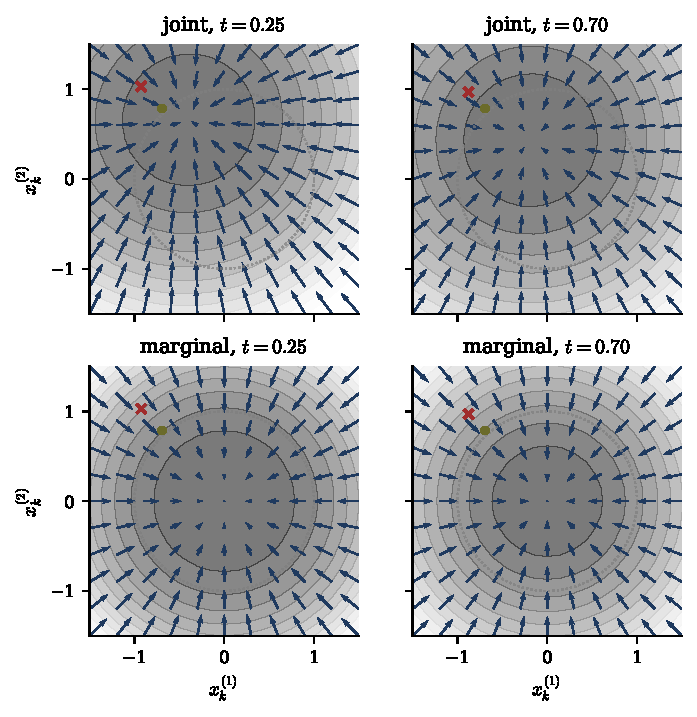
\includegraphics[width=0.78\linewidth]{figures/fig_ring_score_field.pdf}
\caption{Conditional slices of the score block at the central frame,
$k = 10$, one fixed clean trajectory and one fixed standardised noise
realisation, on a $31\times64$ polar grid. Shading is
$\log P_t(x_k\,|\,x_{-k})$, darker for higher density; arrows are the score;
the cross is the noisy observation $x_k$ and the disc the clean frame $a_k$.
Top: the joint conditional field is displaced towards the phase inferred from
the rest of the trajectory. Bottom: the one-frame marginal field stays
ring-symmetric about the origin, because one frame alone does not identify
where along the ring the trajectory is. This is the content of
\eqref{eq:ring-gap} in two dimensions.}
\label{fig:ring-score-field}
\end{figure}

\section{A local linear model}\label{sec:ring-taylor}

The grid calculation is exact but opaque. Expanding around a single rotating
branch turns the model into a linear Gaussian state-space model, whose response
can be computed in closed form.

Take the deterministic reference path $\bar R_k = 1$,
$\bar\Theta_k = \theta_0 + k\omega h$, write
$R_k = 1 + \rho_k$ and $\Theta_k = \bar\Theta_k + \varphi_k$, and let
$e_{r,k}, e_{\theta,k}$ be the moving frame at $\bar\Theta_k$. Rotating the
reference direction by $\varphi_k$ gives, exactly,
$a_k = (1+\rho_k)(\cos\varphi_k\, e_{r,k} + \sin\varphi_k\, e_{\theta,k})$.
Inserting $\cos\varphi = 1 - \varphi^2/2 + O(\varphi^4)$ and
$\sin\varphi = \varphi - \varphi^3/6 + O(\varphi^5)$,
\begin{equation}
  a_k
  = \underbrace{e_{r,k} + \rho_k e_{r,k} + \varphi_k e_{\theta,k}}_{\text{first order}}
    \underbrace{- \tfrac12 \varphi_k^2 e_{r,k}
                + \rho_k\varphi_k e_{\theta,k}}_{\text{second order}}
    + O\big(\norm{(\rho_k,\varphi_k)}^3\big) .
  \label{eq:ring-taylor}
\end{equation}
Keeping the first order, radial deviations move perpendicular to the ring and
angular deviations along the tangent, and to this order the two are decoupled.
The two discarded terms have clear meanings: $-\tfrac12\varphi^2 e_r$ is the
curvature of the circle, which one tangent plane cannot represent, and
$\rho\varphi e_\theta$ is the fact that at larger radius a given angular
deviation moves the point farther. The truncation error is quadratic: for a
pure angular deviation at $\rho = 0$,
$\norm{a_k - \widehat a_k}
= \norm{(\cos\varphi - 1,\ \sin\varphi - \varphi)}
= \varphi^2/2 + O(\varphi^3)$, and retaining the second order reduces it to
$\varphi^3/6$.

Two of the three ingredients are already exactly linear: the radial deviation
follows \eqref{eq:ring-radial-transition} verbatim as an AR(1) chain
$\rho_{k+1} = \alpha_r\rho_k + \sqrt{q_r}\,\xi^{(r)}_k$, and on one unwrapped
angular branch the phase is a random walk
$\varphi_{k+1} = \varphi_k + \sqrt{q_\theta}\,\xi^{(\theta)}_k$. Together with
the linear observation and the linear channel the trajectory is jointly
Gaussian, $x \approx \Nd(\mu_t, \Sigt)$, and its score is
$\score^{\mathrm{lin}}(x,t) = -\Sigt^{-1}(x - \mu_t)$, of exactly the form
studied in Chapter~\ref{ch:gaussian}.

\subsection{When the expansion may be used}\label{sec:ring-taylor-validity}

The truncation error makes the condition quantitative: a $5\%$ error in units
of the ring radius corresponds to $\varphi \approx 0.32$ radians. Two different
quantities must be checked against that number.

The clean spread is small. The angular deviation of the clean process is a
random walk, so after $K-1$ steps its standard deviation is
$\sqrt{q_\theta (K-1)}$, which at the baseline is $0.244$ radians. The clean
trajectory therefore stays within about a quarter of a radian of one rotating
branch over its whole length, and expanding around one branch is reasonable for
the prior.

The posterior spread is what actually matters, because the score involves the
posterior of $\Theta_k$ given the noisy trajectory, and that widens with $t$.
Measured directly as the circular standard deviation of the smoothed angular
posterior at the central frame, averaged over six trajectories, it is $0.085$
radians at $t = 0.03$, $0.248$ at $t = 0.4$, $0.399$ at $t = 0.7$ and $1.62$ at
$t = 2$. The threshold is crossed near $t \approx 0.55$, and
Figure~\ref{fig:ring-taylor} shows the measured score error beginning to grow
just after it.

\begin{remark}[The limits of one tangent plane]\label{rem:ring-taylor}
The expansion is local and phase-conditioned. It cannot represent a posterior
spread over a large arc, several wrapped angular branches, or a multimodal
phase; beyond the crossing point these are not small effects to be bounded but
absent features, and the honest procedure is comparison against the nonlinear
grid calculation. A second limitation is independent of $t$: the reference
phase $\theta_0$ must be estimated from the data, and the resulting error does
not vanish as $t \to 0$. It appears in Table~\ref{tab:ring-taylor} as a floor of
$3$ to $4\%$ on the central-block error even at the smallest diffusion times,
where the angular spread is negligible.
\end{remark}

\begin{figure}[t]\centering
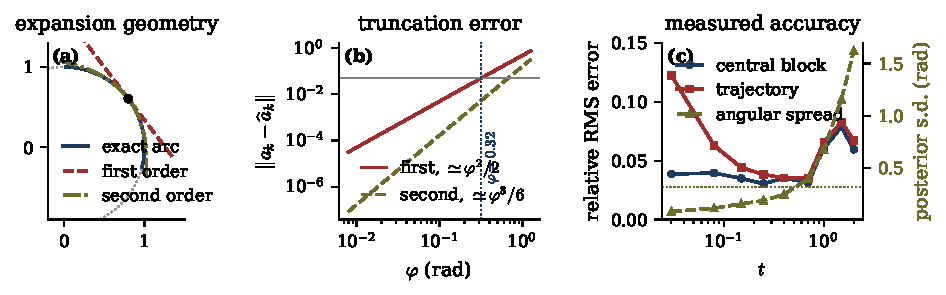
\includegraphics[width=\linewidth]{figures/fig_ring_taylor.pdf}
\caption{The linearisation and its validity. (a) Exact arc, first-order tangent
and second-order parabola through the reference point. (b) Truncation error
against angular deviation: first order is $O(\varphi^2)$ and second order
$O(\varphi^3)$, so a $5\%$ error in units of the ring radius corresponds to
$\varphi \approx 0.32$ radians. (c) Measured relative RMS error of
$\score^{\mathrm{lin}}$ against the nonlinear grid score, left axis, with the
measured circular standard deviation of the smoothed angular posterior on the
right axis; the dotted line is the $0.32$ radian threshold. The error grows
shortly after the posterior spread crosses it.}
\label{fig:ring-taylor}
\end{figure}

\subsection{Reach in closed form}\label{sec:ring-analytic-reach}

The value of the linear model is that its response can be computed by hand,
which turns the statement that the one-step dynamics control the reach into a
formula. For an infinite interior chain the AR(1) prior has Fourier-space
precision $Q_r(\varpi) = (1 + \alpha_r^2 - 2\alpha_r\cos\varpi)/q_r$, the local
observation contributes precision $\lambda_t = e^{-2t}/\Deltat$ at every frame,
and the posterior covariance in Fourier space is
$(\lambda_t + Q_r(\varpi))^{-1}$. Defining $\gamma_r$ by
\begin{equation}
  \cosh\gamma_r = \frac{1 + \alpha_r^2 + q_r \lambda_t}{2\alpha_r} ,
  \label{eq:ring-gamma}
\end{equation}
the inverse transform is a pure exponential,
$C_r(\ell,t) = q_r(2\alpha_r\sinh\gamma_r)^{-1}e^{-\gamma_r|\ell|}$ with
correlation length $\gamma_r^{-1}$; the angular channel is the
$\alpha_r \to 1$ case, with
$\cosh\gamma_\theta = 1 + q_\theta\lambda_t/2$. By
Proposition~\ref{prop:ring-fdt} the score responses are these covariances times
$e^{-2t}/\Deltat^2$. The two factors move in opposite directions: as $t$ grows,
$\lambda_t \to 0$ so $\gamma \to 0$ and the covariance length increases, while
the prefactor drives the score response to zero. This is the mechanism that
\eqref{eq:ring-weighted-reach} was constructed to summarise, here visible in
closed form.

For orientation, the clean process has stationary radial covariance
$(D_r/\kappa)e^{-\kappa h|\ell|}$ and first-harmonic angular coherence
$e^{-D_\theta h |\ell|}$, hence clean scales
$\xi^{\mathrm{clean}}_r = 1/(\kappa h) \approx 1.6$ frames and
$\xi^{\mathrm{clean}}_\theta = 1/(D_\theta h) \approx 637$ frames at the
baseline. The angular coherence length exceeds the length of the trajectory by
more than a factor of $30$: within one data point the phase is essentially a
single coherent quantity, while the radius forgets itself after a couple of
frames. That asymmetry is the prediction tested next.

\section{Measurements}\label{sec:ring-measurements}

At the parameters of Figure~\ref{fig:ring-model}, with $28$ independent clean
trajectories per diffusion time for the response study and $36$ for the window
study, central frame $k = 10$, so $L_{\max} = 10$ and the structureless
ceilings are $\bar\ell = 5.5$ and $\xi^{\mathrm{norm}} = 10$. The radial and
tangential channels are separated by projecting the response blocks on the
moving frame, $J^{rr}_{kj} = e_{r,k}^{\T}J_{kj}e_{r,j}$ and
$J^{\theta\theta}_{kj} = e_{\theta,k}^{\T}J_{kj}e_{\theta,j}$, using the
simulated clean angle as an oracle basis. That is a diagnostic convenience and
not an ingredient of the score; Section~\ref{sec:ring-limits} returns to it.

\begin{table}[t]\centering
\caption{Polar model: cost of dropping temporal context, reach and weighted
reach by channel, and receptive radii. Notation as in
Table~\ref{tab:ring-surrogate}; the structureless ceiling for $\bar\ell$ is
$5.5$.}
\label{tab:ring-response}
\begin{tabular}{@{}rrrrrrrr@{}}
\toprule
$t$ & marginal & $\bar\ell_r$ & $\bar\ell_\theta$
    & $\widetilde\Xi_r$ & $\widetilde\Xi_\theta$
    & $L^{5\%}_r$ & $L^{5\%}_\theta$ \\
\midrule
0.03 & 0.732 & 1.98 & 4.19 & 0.208 & 2.166 & 2 & 9 \\
0.10 & 0.733 & 2.71 & 5.01 & 0.119 & 2.575 & 3 & 9 \\
0.40 & 0.513 & 5.04 & 5.40 & 0.314 & 2.672 & 7 & 9 \\
0.70 & 0.349 & 5.47 & 5.45 & 1.292 & 2.701 & 8 & 9 \\
1.00 & 0.229 & 5.46 & 5.46 & 1.022 & 1.793 & 8 & 9 \\
1.50 & 0.092 & 5.48 & 5.47 & 0.928 & 1.042 & 5 & 7 \\
2.00 & 0.037 & 5.47 & 5.47 & 0.428 & 0.428 & 0 & 0 \\
\bottomrule
\end{tabular}
\end{table}

\paragraph{Joint against marginal.} Replacing the joint score by per-frame
marginal scores costs a relative RMS error of $0.732$ at $t = 0.03$. The error
stays above $0.69$ up to $t = 0.2$, then falls, passing below $0.10$ only near
$t = 1.5$. The nonlinear process therefore agrees with the surrogate that the
effect is not an artefact of the Gaussian construction.

\paragraph{The two channels differ.} At $t = 0.03$ the weighted mean lag is
$1.98$ frames radially against $4.19$ tangentially, and the gap widens once
intensity is included: $\widetilde\Xi_r = 0.21$ against
$\widetilde\Xi_\theta = 2.17$, a factor of ten, where the normalised range
would have reported the same contrast as a factor of $2.5$. This is the
clean-scale prediction of Section~\ref{sec:ring-analytic-reach} confirmed in the
tested regime. The linear model is quantitatively right where it should be: at
$t = 0.03$ it predicts a radial e-folding length of $1.35$ frames against a
measured exponential fit of $1.39$ frames, an agreement to $3\%$. Its
tangential prediction of $4.45$ frames is already comparable to the chain
length, and the measured fit of $6.36$ frames should be read as finite-size
dominated rather than as an estimate of an infinite-system length.

\paragraph{Reach and intensity move in opposite directions.} Between
$t = 0.03$ and $t = 2$ the intensity $I_{\mathrm{off}}$ falls from $8.20$ to
$0.113$, a factor of about $73$, while the weighted mean lag rises from $4.10$
to $5.48$ frames, within $0.4\%$ of the structureless ceiling $5.5$. The
correct reading is not that high-noise frames are strongly coupled, but that
the weak residual coupling is spread evenly along the chain, exactly the
situation of Remark~\ref{rem:ring-ceiling}.

The composite diagnostic resolves the two.
Figure~\ref{fig:ring-diagnostics}(c) reports $\widetilde\Xi$ rising from $1.55$
at $t = 0.03$ to $2.26$ at $t = 0.7$ and falling to $0.43$ at $t = 2$, while
the independently measured receptive radius $L_{5\%}$ takes the values
$8, 8, 9, 9, 9, 6, 0$ across the same diffusion times. Both are non-monotone
and both turn in the same region, whereas $I_{\mathrm{off}}$ decreases
monotonically and $\bar\ell$ and $\xi^{\mathrm{norm}}$ increase monotonically,
so neither elementary diagnostic can indicate a turn at all. Two cautions
belong with this observation: the peaks do not coincide exactly, since in the
surrogate $\widetilde\Xi$ peaks at $t = 1$ and $L_{5\%}$ at $t = 0.7$, and
$\widetilde\Xi$ is a first-moment summary and not a predictor of $L_\epsilon$.

\begin{figure}[t]\centering
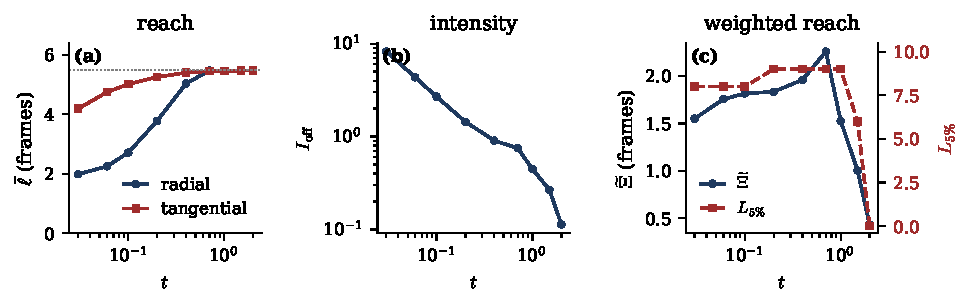
\includegraphics[width=\linewidth]{figures/fig_ring_diagnostics.pdf}
\caption{Diagnostics of the polar model at the parameters of
Figure~\ref{fig:ring-model}, $28$ trajectories per diffusion time.
(a) Weighted mean lag \eqref{eq:ring-mean-lag} by channel; the dotted line is
the structureless ceiling $5.5$, which a completely flat profile would produce.
(b) Absolute cross-frame intensity \eqref{eq:ring-intensity}, which falls by a
factor of about $73$ over the range. (c) The relative weighted reach
\eqref{eq:ring-weighted-reach}, left axis, and the independently measured
receptive radius $L_{5\%}$ of \eqref{eq:ring-window}, right axis. Both are
non-monotone in $t$ and turn near $t = 0.7$.}
\label{fig:ring-diagnostics}
\end{figure}

\paragraph{The receptive field.} At $t = 0.03$ the radial component of the
score reaches $5\%$ accuracy with a window radius of $2$, while the tangential
component needs $9$, nearly the whole trajectory. At intermediate diffusion
times both channels need large windows, and by $t = 2$ a single frame is
already within $5\%$ of the full score, because the cross-frame correction has
become negligible. Read as a possible implication for architecture, in the
guarded sense of Section~\ref{sec:cnn-locality}, this says that the useful
temporal receptive field of a denoiser would depend on the noise level and be
largest in the middle of the schedule. It is a property of this controlled
model, not an established conclusion about trained networks.

\paragraph{The clean dynamics control the low-noise reach.} Increasing $\kappa$
from $0.5$ to $4$ at $t = 0.1$ shortens the radial normalised range from $4.18$
to $2.74$ frames and reduces the nearest-neighbour radial intensity by an order
of magnitude, from $0.35$ to $0.034$: stiffer confinement forgets faster.
Increasing $D_\theta$ from $0.002$ to $0.08$ at the same diffusion time
shortens the tangential normalised range from $8.71$ to $2.96$ frames: faster
dephasing destroys the long tangential channel. Both are what
\eqref{eq:ring-gamma} predicts, and together they answer the second half of the
research question in the tested regime: the reach of the noised score is set by
the one-step clean kernel, modulated by the observation precision $\lambda_t$.

\section{Numerical validation}\label{sec:ring-validation}

Every identity of this chapter is checked against an independently computed
reference, in the protocol of Appendix~\ref{app:repro}.

\begin{table}[t]\centering
\caption{Validation of the rotating-ring computations. The response identity
and the analytic surrogate Jacobian are compared with central finite
differences of the score; the grid check compares two polar resolutions.}
\label{tab:ring-validation}
\begin{tabular}{@{}lrr@{}}
\toprule
check & discrepancy & tolerance \\
\midrule
posterior response identity \eqref{eq:ring-fdt} vs finite differences
  & $6.63\times10^{-9}$ & $10^{-7}$ \\
analytic surrogate Jacobian \eqref{eq:ring-surrogate-score} vs finite differences
  & $9.18\times10^{-6}$ & $10^{-4}$ \\
$41\times128$ against $51\times192$ polar response grid
  & $3.04\times10^{-11}$ & $10^{-7}$ \\
rotation gauge round trip (Lemma~\ref{lem:ring-gauge})
  & $2.22\times10^{-16}$ & $10^{-12}$ \\
clean score on an exact co-rotating ring path
  & $0$ (exact) & $10^{-12}$ \\
\bottomrule
\end{tabular}
\end{table}

\begin{table}[t]\centering
\caption{First-order Taylor score against the nonlinear grid score, $32$
trajectories per diffusion time. The central-block error has a floor of $3$ to
$4\%$ from the estimated reference phase; the growth beyond $t \approx 0.7$
follows the angular posterior spread (Section~\ref{sec:ring-taylor-validity}).}
\label{tab:ring-taylor}
\begin{tabular}{@{}rrrr@{}}
\toprule
$t$ & central RMSE & trajectory RMSE & mean cosine \\
\midrule
0.03 & 0.039 & 0.122 & 0.985 \\
0.15 & 0.035 & 0.044 & 0.997 \\
0.40 & 0.035 & 0.035 & 0.998 \\
0.70 & 0.032 & 0.035 & 0.999 \\
1.00 & 0.061 & 0.065 & 0.992 \\
1.50 & 0.079 & 0.083 & 0.990 \\
2.00 & 0.060 & 0.067 & 0.991 \\
\bottomrule
\end{tabular}
\end{table}

Beyond Table~\ref{tab:ring-validation} the checks include row normalisation of
the transition kernels, global rotation equivariance of the score, stability
under halving the finite-difference step, and the exact vanishing of the clean
surrogate score on a perfect co-rotating ring path. One caveat on grid
convergence: the difference between the $41\times128$ and $51\times192$ grids
is small because the baseline likelihoods and kernels are already smooth at
those resolutions, and a deliberately coarse $11\times24$ grid does show
visible deviations. The production grid is converged for these parameters
rather than trivially grid-independent.

\section{What this chapter establishes}\label{sec:ring-answers}

The clean law is local, and this gives three concrete advantages: the clean
score is assembled from adjacent transition innovations
\eqref{eq:ring-clean-score}; the noised posterior is computable by repeated
one-step operators rather than one integral over $2K$ latent variables; and any
distant influence on $\score_k$ must propagate through a sequence of local
transitions, which is why the parameter sweeps predict the reach from the
one-step kernel. What clean Markovity does not give is locality of the noised
score: for $t > 0$, $\score_k(x,t)$ is not a function of
$x_{k-1}, x_k, x_{k+1}$ alone in either model, because integrating out
uncertain latent states creates posterior correlations at every lag. In the
surrogate that is explicit, the rank-one anchor term of
\eqref{eq:ring-surrogate-score} touching every pair of frames; in the polar
model it is measured.

Both models show the same sequence: a strictly local clean score, then broader
posterior dependence after noising, then the weak universal field $-x$. At
intermediate diffusion times individual frames are noisy enough that distant
context improves the estimate of a clean frame; at large diffusion times the
same context remains statistically present but is no longer materially useful,
because the prefactor $e^{-2t}/\Deltat^2$ of \eqref{eq:ring-fdt} has gone to
zero. The polar process adds a feature the Cartesian surrogate cannot express:
radial information is damped by mean reversion while tangential information
rides a slowly diffusing global phase, so the two score channels have different
reaches and different receptive fields.

Table~\ref{tab:ring-claims} classifies the results in the scheme used
throughout the thesis.

\begin{table}[t]\centering
\caption{Status of the results of this chapter.}
\label{tab:ring-claims}
\begin{tabular}{@{}p{0.52\linewidth}l@{}}
\toprule
result & status \\
\midrule
Joint minus marginal gap \eqref{eq:ring-gap} & exact \\
Posterior response identity \eqref{eq:ring-fdt}
  (Proposition~\ref{prop:ring-fdt}) & exact \\
Gauge reduction and score transformation
  (Lemma~\ref{lem:ring-gauge}) & exact \\
Exact surrogate score and rank-one response
  (Proposition~\ref{prop:ring-exact}) & exact \\
Clean scales $1/(\kappa h)$ and $1/(D_\theta h)$; closed-form reach
  \eqref{eq:ring-gamma} & exact, infinite-chain \\
First-order linearisation \eqref{eq:ring-taylor} and its
  $\varphi \approx 0.32$ validity threshold & assumption-conditional \\
Polar joint score on the $41\times128$ grid & numerical, validated \\
Reach, intensity, weighted reach and receptive radii of
  Tables~\ref{tab:ring-surrogate} and~\ref{tab:ring-response}
  & numerical, one parameter set \\
Non-monotonicity of $\widetilde\Xi$ and $L_{5\%}$ in $t$
  & numerical, observed in the tested regime \\
Receptive field as a reading for architecture & interpretation \\
Behaviour in $K$, unknown rotation class, inferred phase & open \\
\bottomrule
\end{tabular}
\end{table}

\section{Limitations}\label{sec:ring-limits}

\begin{enumerate}
  \item \textbf{One parameter set.} Every number reported here comes from a
  single baseline, with $K = 20$ for the polar model and $K = 30$ for the
  surrogate, and $28$ to $36$ trajectories per diffusion time. Only $\kappa$
  and $D_\theta$ were swept, and nothing is claimed about scaling in $K$.
  \item \textbf{Angular equation.} A constant angular drift was used. A
  different angular drift changes the transition kernel
  \eqref{eq:ring-angular-transition} but not the identities of
  Section~\ref{sec:ring-identities}.
  \item \textbf{Radius positivity.} The shifted process of
  Toolbox~\ref{tb:ring-radial} is formally supported on all of $\R$. At the
  baseline the probability of a negative radius is negligible, but a strict
  model would reflect at the origin or use a positive diffusion.
  \item \textbf{Known rotation.} Lemma~\ref{lem:ring-gauge} assumes $\psi$
  known. An unknown sense of rotation would add a discrete latent variable and
  may produce a speciation phenomenon of the kind discussed in
  Section~\ref{sec:statphys-diffusion}. This is the most interesting single
  extension.
  \item \textbf{Finite trajectory.} At large $t$ the reach diagnostics saturate
  at their structureless ceilings, a finite-size effect and not evidence of a
  divergent correlation length.
  \item \textbf{Oracle projections.} The radial and tangential channels were
  separated using the simulated clean angle; a practical method would infer the
  phase, and that error would enter the projected profiles.
  \item \textbf{Grid approximation.} The polar score is numerically converged
  for these parameters but is not a symbolic closed form.
  \item \textbf{One tangent plane.} The linear model cannot represent wrapped
  or multimodal angular posteriors, which by
  Section~\ref{sec:ring-taylor-validity} is the regime beyond
  $t \approx 0.55$.
\end{enumerate}

The immediate extensions are to vary $K$ systematically, to infer the angular
phase rather than use an oracle basis, to add an unknown rotation class, and to
test whether a time-dependent local architecture with receptive field
$L_\epsilon(t)$ can match the full score.
